\documentclass[12pt,a4paper,english]{article}

\usepackage[left=2cm, top=3cm, text={17cm, 24cm}]{geometry} 
\usepackage[pdftex]{graphicx}
\usepackage[utf8]{inputenc}
\usepackage{tabularx}
\usepackage[hyphens]{url}
\usepackage[unicode, colorlinks=true, hypertexnames=false, allcolors=blue]{hyperref}
\usepackage{xcolor}
\usepackage{times}
\usepackage{amsmath}


\newcommand{\todo}[1]{\textcolor{red}{[[\textbf{TODO} \textbf{#1]]}}}

\begin{document}
    \begin{titlepage}
        \begin{center}
            \vspace*{1cm}
        
            \begin{figure}[h!]
                
\includegraphics[scale=0.12]{VUT-FIT-logo-en.png}
            \end{figure}
            \vspace{1.5cm}

            \Large{\textbf{Epidemiological model on macro level}} \\
            \large{Modelling and Simulation}

            \vspace{0.5cm}
                
            \vspace{1.5cm}
            
            \textbf{Abramov Mikhail (xabram00)} \\
            \textbf{Pavel Yadlouski (xyadlo00)} 

            \vfill
                
            \vspace{0.8cm}
        
            Brno University of Technologies\\
            November, 2020
                
        \end{center}
    \end{titlepage}

    \tableofcontents
    \newpage

    \section{Introduction}
    The first aim of this project is to determine the possibilities for determining the value of the effectiveness of various restrictive measures taken by the government of the Czech Republic for the period from September 1, 2020 till the last day of the project - December 7, 2020.

    The second aim is to create a predictive model for determining the number of persons who have illness in the same time, persons who have been ill or otherwise have immunity
    % \todo{перенести это в пункт с допущениями когда он будет?}, the number persons who will not be able to resist the disease and as a result will die. 
    % \todo{Данные показатели очень важны для принятия решения о: 1) вводе новых мер 2) отмене старых мер 3) подготовке больничных мест, т.к. при их нехватке смертность значительно возрастает 4) оценка последствий как мер так и самой болезни}
    
    Used model contains different scenarios of quarantine precautions (using different types of lockdown).
    Based on simulations of this scenarios, influence of particular scenario is shown. 
    As an experiment, theoretical scenarios from the article and current lockdown type in Czech Republic are analyzed.

    \subsection{Contributors}    
    This project is solved by team of two students: Abramov Mikhail and Pavel 
    Yadlouski.
    
    \subsection{Model validation}
    Results of theoretical scenarios simulation are compared with reference results from the article. 
    The article by itself was subjected to critical analysis and minor formulas adjustments.
    Experiment with lockdown type in Czech Republic is compared with reality:) 
    
    % \todo{Для достижения поставленных задач было выбрано исследование - ссылочка. Данная статья использует модифицированную модель СИРД для оценки изучения и оценки различных моделей карантинных мер. 
    %       Данная модель без модификаций имеет довольно широкое распространенние и часто используется для описания распространения заболеваний. (можно бахнуть несколько других статей как подтверждение что модель часто импользуется)
    %       Валидация корректности имплементации данной модели была сверена с результатами представленными в статье а сама статья подвержена критическому анализу и незначительной корректировке формул. <- DONE
    %       Далее для определения эффективности мер принятых чешским правительство (надо накидать ссылочек на меры мб) использовалась модель подготовленная в соответствии с приведенной выше статьей и статистика по заболеванию Ковид из официальных источников (ссылочка на ковид стат).
    %       За валидацию корректности наших гипотетических оценок принято соответствие основных трендов развития модели с данныими официальной статистики}.
    

    \newpage
    \section{Topic analysis}

    As epidemic situation in the world become worth with time, there is need to take appropriate precautions based on mathematical models and simulation.
    Epidemiological model can be described as by stochastic as by deterministic model.
    Stochastic model can describe epidemics on micro level.
    For example on micro level time period between visitors came to the market is stochastic.
   
    But on macro level with large populations epidemics is described using deterministic model.
    In this model each individual of the population is assigned to different subgroup.
    And each subgroup represents a specific stage of the epidemic.
    The transition rates from one class to another are mathematically expressed as derivatives, this way model is defined by differential equations.
    In any time of the simulation following equation should valid:
    $$P = \sum_{n = 1}^{n} S^t_n$$
    where $P$ is size of initial and $S^t_n$ is size of the subgroup $S_n$ in the time $t$. 

    One of the base mathematical model for simulation of expansion of the epidemic is SIR\footnote{\href{https://en.wikipedia.org/wiki/Compartmental\_models\_in\_epidemiology}{https://en.wikipedia.org/wiki/Compartmental\_models\_in\_epidemiology}} model. 
    SIR model is the simplest compartment methods that can be extended using different methodologies.
    This method compares three values:
    \begin{enumerate}
        \item \textbf{S} -- the number of \textbf{s}usceptible individuals
        \item \textbf{I} -- the number of \textbf{i}nfectious individuals.
        \item \textbf{R} -- the number of \textbf{r}emoved (and immune) or deceased individuals
    \end{enumerate} 

    \subsection{Sources}
    The necessary information to research this topic was found in scientific articles from IRCACS-International Research Center for Applied Complexity Sciences in  Colombia written by Danny Ibarra-Vega\cite{math_article}.

    \subsection{Approaches}
    For more complex view of system behavior, a mathematical model has been adopted with the Systems Dynamics(SD) methodology\footnote{\href{https://en.wikipedia.org/wiki/System\_dynamics}{https://en.wikipedia.org/wiki/System\_dynamics}}.
    The core of this methodology is that SD models solve the problem of simultaneity (mutual causation) by updating all variables in small time increments with positive and negative feedbacks and time delays structuring the interactions and control.
    
    Used SD model extends basic SIR model with separating the number of recovered and deceased individuals into two variables and addition of auxiliary and state variables that represent hospital capacity, contacts, contacts with infected. 
    As a result, there is a model of 4 stock variables and 4 corresponding differential equations (\ref{eq:quations}).

    \newpage
    \section{Concept model} \label{conc_model}
    In the model, we proceed from the assumption that immunity is stable and guarantees the absence of recurrent disease for the duration of research period. 
    
    \begin{center}
        \begin{figure}[ht!]
            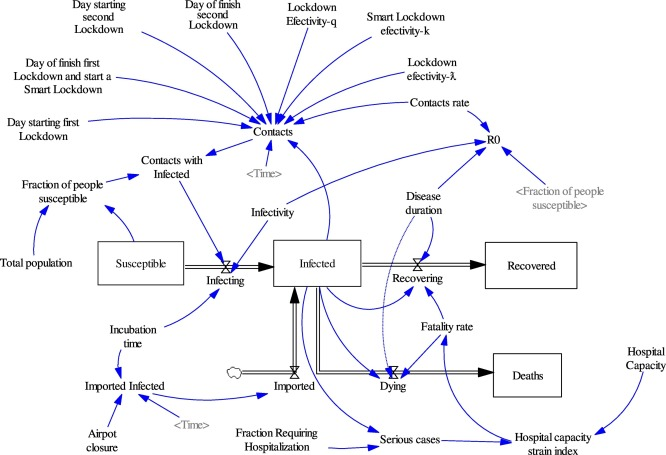
\includegraphics[scale=1]{1-s2.0-S0048969720324347-gr1.jpg}
            \caption{Stock and flows diagram}
            \label{fig:graph}
        \end{figure}
    \end{center}
    
    The diagram \ref{fig:graph}  from the reference article shows how each stock variable (susceptible, infectious, removed, deaths) is connected and influenced by other stock and auxiliary variable.
    Also 
    Auxiliary variables are constructed from bibliographic references or some estimated.
    
    \begin{table}[h!]
        \centering
        \begin{tabularx}{\textwidth}{|c|c|c|X|}
            \hline
            Name & Initial value & Units & Reference \\
            \hline
            Susceptible	                        & 100,000 &	People & Assumed\\
            Incubation time	                    & 5	 &  Days & Wu et al. (2020)\\
            Disease duration                    & 14	&  Days & Wu et al. (2020)\\
            Fraction requiring hospitalization	& 13  & \% & WHO report 73 (2020), Li et al. (2020) \\
            Infectivity	                        & 0.025 & Dimensionless & Estimated with RO \\
            Contacts rate	                    & 70   & Contacts/person & Assumed \\
            Hospital capacity	                & 1000 & Beds & Assumed \\
            Fatality rate	                    & 3	   & \% & WHO report 73 (2020), Wu et al. (2020) \\
            \hline
        \end{tabularx}
        \caption{Initial conditions \cite{math_article}}
        \label{tab:init_vars}
    \end{table}
    
    Meaning and notation of individual variable is explained in the table \ref{tab:not_var}

    \begin{table}[h!]
        \begin{center}
            \begin{tabular}{|c|c|c|}
                \hline
                Type of variable & Parameter & Notation \\
                \hline
                Auxiliary & Contacts rate                      & $\mu$  \\
                Auxiliary & Fatality rate                      & $Fr$ \\
                Auxiliary & Hospital capacity strain index     & $HiC$ \\
                Parameter & Incubation time                    & $it$ \\
                Parameter & Disease duration                   & $Dd$ \\
                Parameter & Fraction requiring hospitalization & $Fh$ \\
                Parameter & Infectivity                        & $\beta$ \\
                Parameter & Hospital capacity                  & $HC$ \\
                Parameter & Lockdown effectivity               & $\lambda$ \\
                Parameter & Smart lockdown effectivity         & $k$ \\
                Parameter & Post lockdown effectivity          & $q$ \\
                Parameter & Serious cases                      & $SC$  \\
                Parameter & Hospital capacity                  & $HC$ \\
                Stock     & Susceptible                        & $S$ \\
                Stock     & Infected                           & $I$ \\
                Stock     & Recovered                          & $R$ \\
                Stock     & Deaths                             & $D$ \\
                \hline
            \end{tabular}
        \end{center}
        \caption{Notation and variables \cite{math_article}}
        \label{tab:not_var}
    \end{table}

    Mathematical model of epidemic is
    \begin{subequations} \label{eq:quations}
        \begin{align*} 
            \frac{dS}{dt} &= - \frac{\beta Ci}{it}  \\ \\
            \frac{dI}{dt} &= \frac{\beta C}{it} - \frac{I}{Dd} * (1 - Fr)\\ \\
            \frac{dR}{dt} &= \frac{I}{Dd} * (1 - Fr)\\ \\
            \frac{dD}{dt} &= \frac{I}{Dd} * (Fr)
        \end{align*}
    \end{subequations}


    During implementation of the model from the article, we found out that some variables in auxiliary equations are not defined in the article. 
    For example variable F is not present in the article. Using addition source article from Harvard University \cite{Harvard}. We determined that
    variable F is Si divideed on the total number of population, otherwise we decided not to use additional variable for population and decided to use
    initial value of Susceptibles as total population. 
    
    So, auxiliary equations that we used have following form
    \begin{subequations}
        \begin{align*} 
            Ci  &= C *F \\
            F   &= \frac{S}{S_{int}} \\ 
            HiC &= \frac{SC}{HC} \\
            SC  &= I * Fh \\
            Fr  &=    
            \begin{cases}
                3\% \; if \; HiC < 5 \\
                7\% \; if \; 5 < HiC < 30 \\
                10\% \; if \; HiC > 30
            \end{cases}
        \end{align*}
    \end{subequations}

    Influence of lockdown scenarios is described in the following way
    \begin{subequations}
        \begin{align*} 
            C  &=    
            \begin{cases}
                I * \mu \; if \; t \leq  t_1 \\
                I * \mu * \lambda \; if \; t_1 < t \leq t_2 \\
                I * \mu * k \; if \; t_2 < t \leq t_3 \\
                I * \mu * q \; if \; t_3 < t \leq t_4
            \end{cases}
        \end{align*}
    \end{subequations}

    \section{Experiment}
    
    \todo{Misha napishy suda}

    \section{Conclusion}
    \todo{Co se naucili}
    
    \todo{Doporuceni}

    \todo{Experiment with other country}

    \clearpage
	\bibliographystyle{abbrv}
	\bibliography{citation}
\end{document}